\documentclass[pdftex,letterpaper,12pt]{report}
\usepackage{thesis}
\usepackage{amsmath}
\usepackage{amssymb}
\usepackage{amsthm}
\usepackage{mathtools}
\usepackage{bm}
\usepackage{gensymb}
\usepackage{wasysym}
\usepackage{mathtools}
\usepackage{physics}
\usepackage{empheq}
\usepackage{cases}
\usepackage{rotating}
\usepackage{subfig}
\usepackage{caption}
\captionsetup{labelfont=bf} 
\captionsetup[subfloat]{position=top,singlelinecheck=off,justification=raggedright,font=bf,labelfont=large,labelformat=simple,captionskip=-2mm}
\usepackage{float}
\usepackage{enumitem} 
\usepackage[toc,page]{appendix}






\begin{document}
	
\begin{equation}
\frac{1}{T_{r1}}=\frac{R^{4}|\nabla\Omega_{z}|^{2}}{r^{2}(1+s^{2})^{2}D}=\frac{|\nabla B_{z}|^{2}D}{B^{2}(1+s^{2})^2}
\end{equation}

Eq.\ref{InitialSpinup} haha

\section{section}
\subsection{sub}
\subsubsection{sub1}
\subsubsection{sub2}

\begin{figure}[H]
	\centering
	\resizebox{0.91\textwidth}{!}{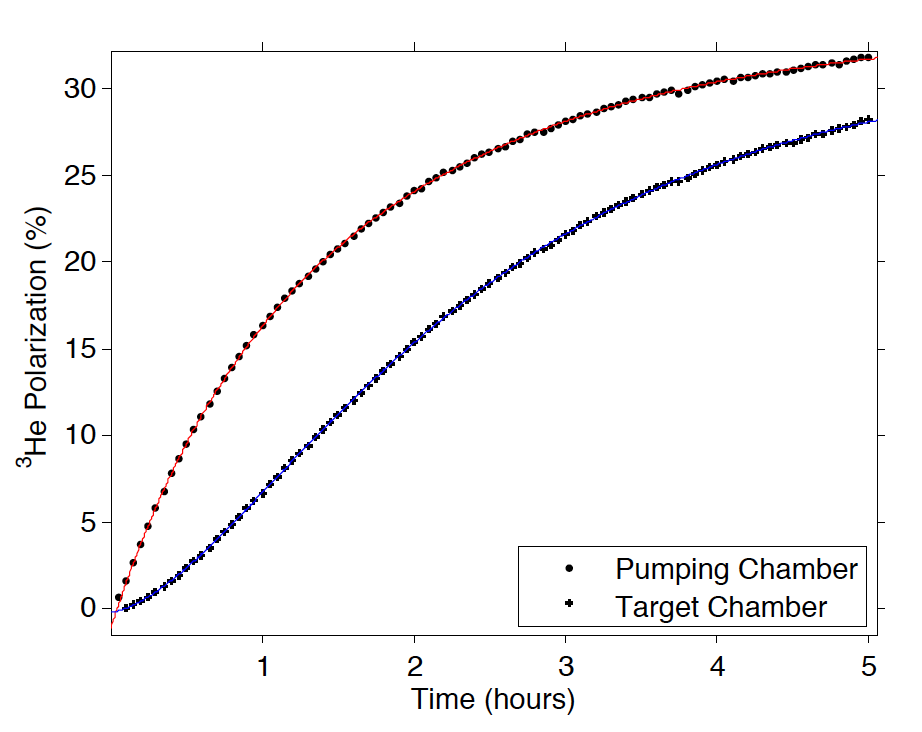
\includegraphics{BradySpinup.png}}
	\caption{{\bf $^{3}$He polarization as a function of time for both the pumping chamber and the target chamber. The top curve is the pumping chamber and the bottom curve is the target chamber.}}
	\label{BradySpinup}
\end{figure}

\emph{et al.}
$\Delta F=\pm1$
$\vec{S}$

\addcontentsline{toc}{chapter}{Bibliography}
\bibliography{ref}

\end{document}